Multicore architectures 
cache system
sharing and false sharing
existing tools for false sharing
limitations
contributions
structures

Modern computer systems, such as server nodes, desktops, and smart phones, employ multiple cores to explore high parallelism. To bridge the speed gap between CPU and main memory, multi-level cache hierarchies are used to block data for fast accesses. Typically in the memory hierarchy, there are private layers associated with each core and shared layers between cores. For example, Intel Sandy Bridge processors have private L1 and L2 caches, as well as shared L3 caches. Moreover, IBM POWER8 have L1, L2 private caches, and L3, L4 shared caches.
To facilitate programming and guarantee the correctness, there are complex cache coherency protocols~\cite{} implemented in the hierarchy.

The complex memory hierarchies in multi-core systems may suffer from various performance issues, such as poor data locality~\cite{}, intensive cache contention~\cite{}, and bandwidth underutilization~\cite{}. Among them, false sharing is a common programming flaw that can significant hurt a parallel program's performance and scalability. False sharing occurs between threads, when these threads (1) run on cores with private caches, (2) access different words of a cache line, and (3) at least one access is a write. Given the cache coherence protocol, threads with writing the words keep invalidating the cache line in all private caches and flushing the data to the shared caches. Thus, when some threads use the data, they need to load the data from the shared cache, rather than the fast private one.

%Multicore processors are ubiquitous, from phones, desktops, to high-end servers.
%False sharing occurs when multiple tasks, running on different cores with private L1 caches, access logically independent words in the same cache line. When a thread modifies data of a cache line, the underlying cache coherence protocol (inside hardware) silently invalidates the duplicates of this cache line on other cores. Unnecessary synchronizations caused by false sharing can dramatically degrade the performance of parallel software by up to an order of magnitude ~\cite{falseshare:effect}. A simple example shown in Figure~\ref{fig:penalty} also exemplifies this catastrophic performance effect of false sharing. Figure~\ref{} shows how false sharing occurs in a typical multi-core platform.


%The hardware trend, including adding more cores into the same machine, introducing the Non-Uniform-Memory-Access (NUMA) architecture, or increasing the size of a cache line, will further degrade the performance of false sharing problems, making the task of detecting even more urgent. 

\begin{figure*}[htbp]
\centering
\subfigure[Parallel Programs]{%
   \label{fig:penaltycode}
   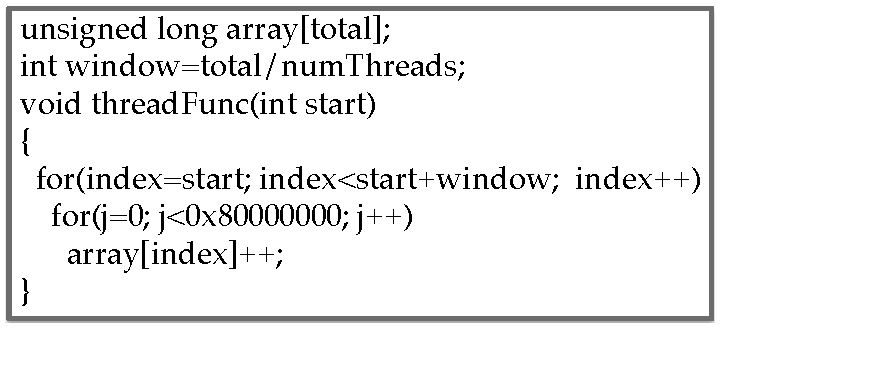
\includegraphics[width=2.8in]{figure/fscode}

}%
\hspace{30pt}
\subfigure[Performance Degradation]{%
   \label{fig:penaltyfig}
   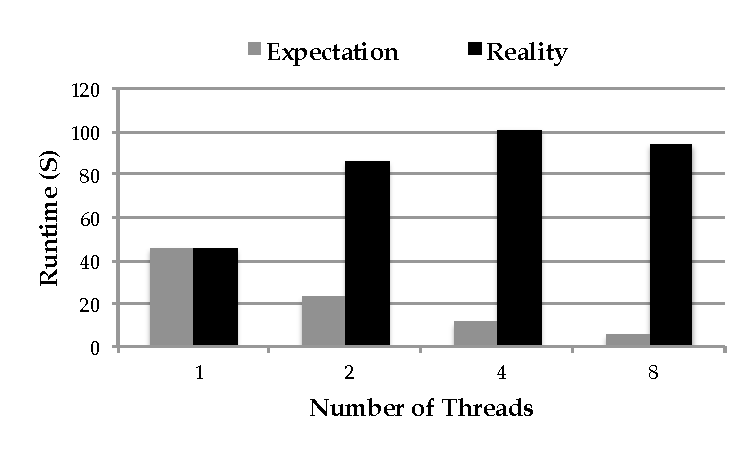
\includegraphics[width=2.4in]{figure/penalty}
}
\caption{
A false sharing example inside a multithreaded program (a) causes $13\times$ performance degradation (b) on a 8-core machine.
\label{fig:penalty}}
\end{figure*}

% Now we will talk about existing tools. 
As a concrete example, as shown in Figure~\ref{fig:penalty}, careless code design can lead to false sharing: multiple threads access adjacent elements of {\tt array} that reside in the same cache line. When parallelize this loop with threads, one can see from Figure~\ref{fig:penaltyfig} that the scalability (in red) is much worse than expected (in green). Therefore, it is important to eliminate false sharing to obtain high performance and scalability. 
Unlike true sharing, false sharing is avoidable. As threads unnecessarily share the same cache line, we can pad the data to force each thread access a different cache line. Although the solution for false sharing is straightforward, detecting it is difficult and even impossible with manual effort only, especially for a code with hundreds of thousands of lines. There is a demand for tool to pinpoint false sharing and provide insightful optimization guidance.

However, existing generic performance tools do not provide details about false sharing. For example, profilers such as gprof~\cite{gprof}, HPCToolkit~\cite{}, TAU~\cite{}, and VTune~\cite{} report time consumption and cache miss counts, but do not point that the long running time and large amount of cache misses are caused by false sharing or not. However, existing special tools for detecting false sharing also lacks in several ways. First, some tools~\cite{falseshare:binaryinstrumentation1,detect:ptu,detect:intel,falseshare:binaryinstrumentation2,DProf, qinzhao, OSdetection, mldetect, Wicaksono11detectingfalse, openmp} do not distinguish true and false sharing, leaving much burden for programers to fix. Second, some tools~\cite{falseshare:binaryinstrumentation1,falseshare:binaryinstrumentation2,falseshare:simulator, Predator} introduce much performance overhead, preventing them from practical usage. Third, some tools require special OS support~\cite{OSdetection} or only work on a special type of applications~\cite{sheriff}. Fourth, no tool assesses the benefit from eliminating the false sharing, thus many efforts may lead to trivial performance improvement.

\vspace{0.2in}

To address these issues, we develop \cheetah{} with the following three contributions:
\begin{itemize} 
\item \cheetah{} can report precise information about false sharing problems. Like those precise tools, e.g. Sheriff~\cite{sheriff} and Predator~\cite{Predator}, it will pinpoint the lines of code where those variables or objects have false sharing problems. More than that, \cheetah{} can further pinpoint statements exercising false sharing problems, which can help programmers to fix found problems. 

\sloppy
\item Leveraging on hardware performance counters, \cheetah{} significantly reduces the performance overhead of detection, with only 5\% average performance overhead and 10\% maximum overhead. The performance overhead is similar to recent work~\cite{mldetect, openmp}, but with more precise information and more effectiveness.
  
\item Different with all existing tools, \Cheetah{} can predict the performance impact of false sharing instances based on latency information provided by performance monitoring units. By ruling out non-important cases, \Cheetah{} can avoid unnecessary manual effort as much as possible. 
\end{itemize}
\cheetah{} is a compiler-independent tool that works on fully optimized binaries. To evaluate \cheetah{}, we apply it to a number of well-known benchmarks from Phoenix and Rodinia suites. Experiments show that \cheetah{} can efficiently and effectively guide us fix false sharing problems with significant performance improvement.

The remainder of this paper is organized as follows. Section~\ref{sec:overview} introduces the background of false sharing and \cheetah{}'s basic idea. Section~\ref{sec:implement} describes implementations in detail. Section~\ref{sec:eval} presents experimental results, including effectiveness, performance overhead, and memory overhead. Section~\ref{sec:relatedwork} discusses some related work and Section~\ref{sec:relatedwork} concludes this paper. 



